\section{Introduction:}

An operational amplifier, or op-amp, is a very high gain differential amplifier with high input impedance and low output impedance. Typical uses of the operational amplifier are to provide voltage amplitude changes (amplitude and polarity), oscillators, filter circuits, and many types of instrumentation circuits. An op-amp contains a number of differential amplifier stages to achieve a very high voltage gain. \hfill \break

Figure 2.0 shows a basic op-amp with two inputs and one output as would result using a differential amplifier input stage. 

\begin{figure}[H]
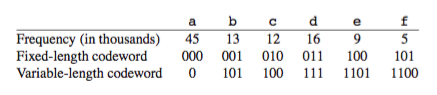
\includegraphics[scale=.6]{1.png}
\centering \linebreak \linebreak Figure 2.0: Basic op-amp.
\end{figure}

\subsection{Practical OP-AMP circuits:}

The op-amp can be connected in a large number of circuits to provide various operating characteristics. In this section, we cover a few of the most common of these circuit connections.

\subsubsection{Inverting Amplifier:}

The most widely used constant-gain amplifier circuit is the inverting amplifier, as shown in Figure 2.1.1.0. The output is obtained by multiplying the input by a fixed or constant gain, set by the input resistor $R_{1}$ and feedback resistor $R_{f}$ this output also being inverted from the input. The we can write: \hfill \break

\begin{ceqn}
\begin{align*}
V_{0}\ =\ -\ \frac{R_{f}}{R_{1}} \cdot V_{1}
\end{align*}
\end{ceqn} \hfill 

\begin{figure}[H]

\includegraphics[scale=.6]{2.png}
\centering \linebreak \linebreak Figure 2.1.1.0: Inverting constant-gain multiplier.
\end{figure}

\subsubsection{Non-Inverting Amplifier:}

The connection of Figure 2.1.2.0 shows an op-amp circuit that works as a non-inverting amplifier or constant-gain multiplier. It should be noted that the inverting amplifier connection is more widely used because it has better frequency stability. To determine the voltage gain of the circuit, we can use the equivalent representation shown in Figure 2.1.2.1. \hfill \break

{\bfseries\itshape\color{airforceblue}{Note:}} {\itshape\color{airforceblue}{The voltage across $R_{1}$ is $V_{1}$ since $V_{i}\ \cong\ 0\ V$. This must be equal to the output voltage, through a voltage divider of $R_{1}$ and $R_{f}$, so that:

\begin{ceqn}
\begin{align*}
V_{1}\ =\ \frac{R_{1}}{R_{1}\ +\ R_{f}} \cdot V_{0}
\end{align*}
\end{ceqn}}} \hfill

The we can say that: \hfill \break

\begin{ceqn}
\begin{align*}
V_{0}\ =\ (\ 1\ +\ \frac{R_{f}}{R_{1}}\ )\ V_{1}
\end{align*}
\end{ceqn} \hfill

\begin{multicols}{2}
\begin{figure}[H]
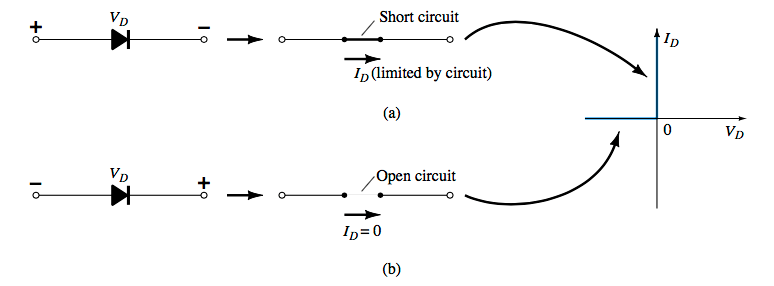
\includegraphics[width = 8cm, height = 5cm]{3.png}
\centering \linebreak \linebreak Figure 2.1.2.0: Non-inverting constant-gain multiplier.
\end{figure}

\begin{figure}[H]
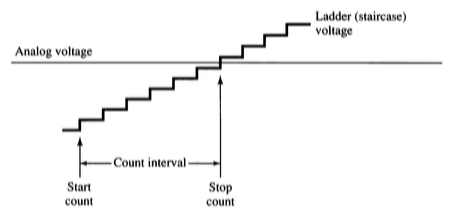
\includegraphics[width = 8cm, height = 5cm]{4.png}
\centering \linebreak \linebreak Figure 2.1.2.1: Sub-circuit of Figure 2.1.2.0.
\end{figure}
\end{multicols}

\subsubsection{Unity Follower:}


The unity-follower circuit, as shown in Figure 2.1.3.0, provides a gain of unity (1) with no polarity or phase reversal. From the equivalent circuit Figure 2.1.3.1 it is clear that: \hfill \break

\begin{ceqn}
\begin{align*}
V_{0}\ =\ V_{1}
\end{align*}
\end{ceqn} \hfill

And that the output is the same polarity and magnitude as the input. The circuit operates like an emitter- or source-follower circuit except that the gain is exactly unity. \hfill \break

\begin{multicols}{2}
\begin{figure}[H]
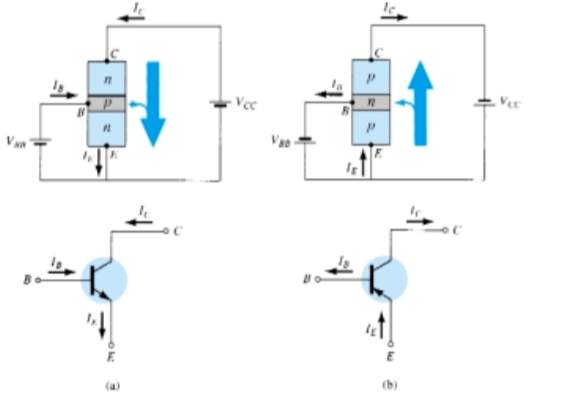
\includegraphics[width = 8cm, height = 5cm]{5.png}
\centering \linebreak \linebreak Figure 2.1.3.0: Unity follower.
\end{figure}

\begin{figure}[H]
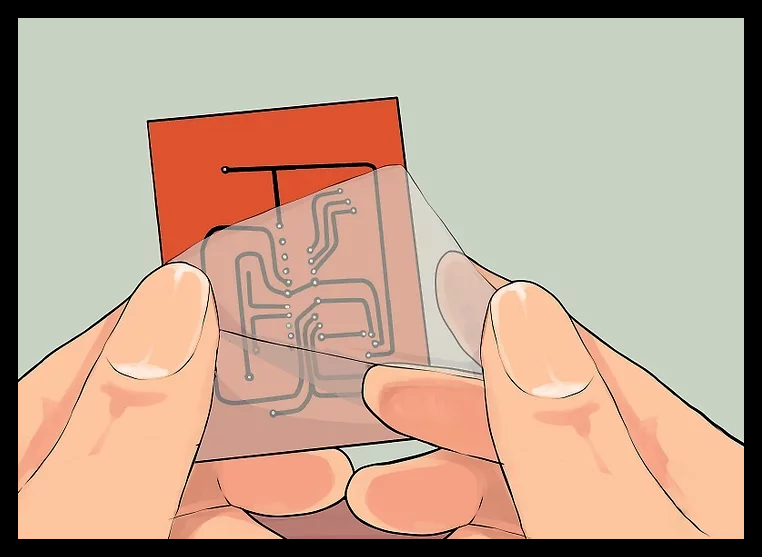
\includegraphics[width = 8cm, height = 5cm]{6.png}
\centering \linebreak \linebreak Figure 2.1.3.1: Virtual-ground equivalent circuit.
\end{figure}
\end{multicols}

\pagebreak

\subsubsection{Summing Amplifier:}


Probably the most used of the op-amp circuits is the summing amplifier circuit shown in Figure 2.1.4.0. The circuit shows a three-input summing amplifier circuit, which provides a means of algebraically summing (adding) three voltages, each multiplied by a constant-gain factor. Using the equivalent representation shown in Figure 2.1.4.1, the output voltage can be expressed in terms of the inputs as:

\begin{ceqn}
\begin{align*}
V_{0}\ =\ -\ ( \frac{R_{f}}{R_{1}} \cdot V_{1} \ +\ \frac{R_{f}}{R_{2}} \cdot V_{2} \ +\ \frac{R_{f}}{R_{3}} \cdot V_{3}\ )
\end{align*}
\end{ceqn} \hfill

In other words, each input adds a voltage to the output multiplied by its separate constant-gain multiplier. If more inputs are used, they each add an additional component to the output.

\begin{multicols}{2}
\begin{figure}[H]
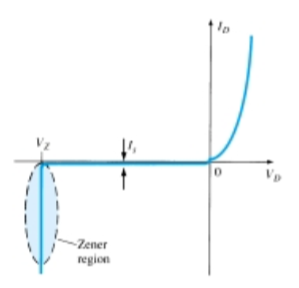
\includegraphics[width = 8cm, height = 5cm]{7.png}
\centering \linebreak \linebreak Figure 2.1.4.0: Summing amplifier.
\end{figure}

\begin{figure}[H]

\includegraphics[width = 8cm, height = 5cm]{8.png}
\centering \linebreak \linebreak Figure 2.1.4.1: Virtual-ground equivalent circuit.
\end{figure}
\end{multicols}

\subsubsection{Differentiator:}

A differentiator circuit is shown in Figure 2.1.4.0. While not as useful as the circuit forms covered above, the differentiator does provide a useful operation, the resulting relation for the circuit being: \hfill \break
 
\begin{ceqn}
\begin{align*}
v_{0}\ (\ t\ )\ =\ -\ R \cdot C\ (\ \frac{dv_{1}\ (\ t\ )}{dt}\ )
\end{align*}
\end{ceqn} \hfill

where the scale factor is -RC. \hfill \break

\begin{figure}[H]
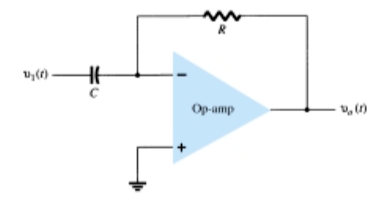
\includegraphics[width = 8cm, height = 5cm]{9.png}
\centering \linebreak \linebreak Figure 2.1.5.0: Differenciator circuit.
\end{figure}

\pagebreak

\subsubsection{Integrator:}

So far, the input and feedback components have been resistors. If the feedback component used is a capacitor, as shown in Figure 2.1.6.0, the resulting connection is called an integrator. The virtual-ground equivalent circuit Figure 2.1.6.1 shows that an expression for the voltage between input and output can be derived in terms of the current {\bfseries\itshape I}, from input to output. Recall that virtual ground means that we can consider the voltage at the junction of {\bfseries\itshape R} and {\bfseries\itshape $X_{C}$} to be ground (since $V_{i}\ \cong\ 0\ V$.) but that no current goes into ground at that point. The capacitive impedance can be expressed as: \hfill \break

\begin{ceqn}
\begin{align*}
X_{C}\ =\ \frac{1}{j \cdot \omega \cdot C}\ =\ \frac{1}{s \cdot C}
\end{align*}
\end{ceqn} \hfill

\begin{multicols}{2}
\begin{figure}[H]
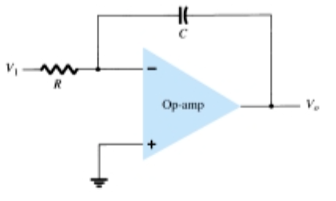
\includegraphics[width = 8cm, height = 5cm]{10.png}
\centering \linebreak \linebreak Figure 2.1.6.0: Integrator.
\end{figure}

\begin{figure}[H]
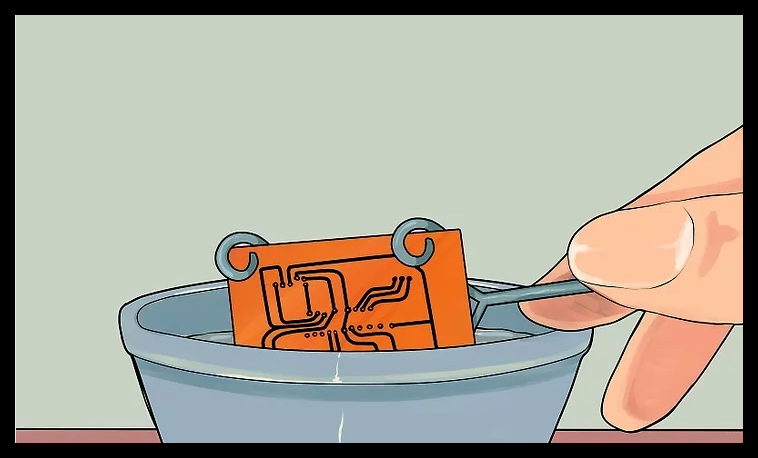
\includegraphics[width = 8cm, height = 5cm]{11.png}
\centering \linebreak \linebreak Figure 2.1.6.1: Virtual-ground equivalent circuit.
\end{figure}
\end{multicols} \hfill

For $v_{0}\ (\ t\ )$: \hfill \break

\begin{ceqn}
\begin{align*}
v_{0}\ (\ t\ )\ =\ -\ \frac{1}{R \cdot C}\ \int\ v_{1}\ (\ t\ )\ dt
\end{align*}
\end{ceqn} \hfill

\pagebreak
